%\documentclass[dvipdfmx]{beamer}      % platex の場合
\documentclass[handout]{beamer}        % lualatex の場合
\usepackage{mySld}

\begin{document}
\title{基礎コンピュータ工学\\第2章 情報の表現\\
       (パート5:小数や文字の表現と補助単位)}
\date{}

\begin{frame}
  \titlepage
  \centerline{\url{https://github.com/tctsigemura/TecTextBook}}
  \vfill
  \centerline{本スライドの入手:
    \raisebox{-7mm}{\includegraphics[scale=0.3]{../Img/QRs2_4.png}}}
\end{frame}

%==============================================================================
%\begin{frame}
%  \frametitle{}
%\end{frame}

\section{情報の表現}
%==============================================================================
\begin{frame}
  \frametitle{2進数による小数の表現}
  \emph{固定小数点方式}(小数点の位置を\emph{約束}する.)
  \vfill
  \begin{quote}
    \begin{minipage}{0.4\columnwidth}
      $00.00_2 = 0.0_{10}$  \\
      $00.01_2 = 0.25_{10}$  \\
      $00.10_2 = 0.5_{10}$  \\
      $00.11_2 = 0.75_{10}$  \\
      $01.00_2 = 1.0_{10}$  \\
      $01.01_2 = 1.25_{10}$  \\
      $01.10_2 = 1.5_{10}$  \\
      $01.11_2 = 1.75_{10}$  \\
      $10.00_2 = 2.0_{10}$  \\
      ...\\
      $11.11_2 = 3.75_{10}$
    \end{minipage}
    \begin{minipage}{0.5\columnwidth}
      \emph{桁の重み}
      \begin{itemize}
      \item 小数点から左に進むと2倍
        $001.0000_2 = 1.0_{10}$ \\
        $010.0000_2 = 2.0_{10}$ \\
        $100.0000_2 = 4.0_{10}$ \\
        \vspace{1ex}
      \item 小数点から右に進むと1/2倍\\
        $000.1000_2 = 0.5_{10}$ \\
        $000.0100_2 = 0.25_{10}$ \\
        $000.0010_2 = 0.125_{10}$ \\
        $000.0001_2 = 0.0625_{10}$
      \end{itemize}
    \end{minipage}
  \end{quote}
\end{frame}

%==============================================================================
\begin{frame}
  \frametitle{固定小数点方式2進数 →  10進数}
  桁の重みを合計する.
  \begin{align}
    10.01_2 &= 1 \times 2 + 0 \times 1 + 0 \times 1/2 + 1 \times 1/4 \notag\\
            &= 2 + 0 + 0 + 1/4 \notag\\
            &= 2 + 0.25 \notag\\
            &= 2.25 \notag
  \end{align}
  \vfill
  \emph{問題12:}2進数を10進数に変換しなさい.
  \begin{enumerate}
  \item[1)] $0101.1010_2$
  \vfill
  \item[2)] $0011.0011_2$
  \vfill
  \item[3)] $0100.0101_2$
  \vfill
  \item[4)] $1010.1111_2$
  \end{enumerate}
\end{frame}

%==============================================================================
\begin{frame}
  \frametitle{10進数 →  固定小数点方式2進数}
  \centerline{\parbox{0.8\columnwidth}{\small
      \begin{center}
\begin{tabular}{ r l  l r}
\multicolumn{1}{c}{2進数} &  ~~~$\times 2$は~~~ & \multicolumn{2}{c}{10進数}\\
$0.101_2$ &        左シフ       &           & $0.625$ \\
\multicolumn{1}{c}{$\swarrow$} &   トと同じ     & $\times$  &     $2$ \\
\cline{3-4}
$1.010_2$      &                &           & $\underline{1}.250$ \\
&&&\\
\multicolumn{1}{c}{2進数} &  ~~~$\times 2$は~~~ & \multicolumn{2}{c}{10進数}\\
$0.010_2$ &        左シフ       &           & $0.250$ \\
\multicolumn{1}{c}{$\swarrow$} &   トと同じ     & $\times$  &     $2$ \\
\cline{3-4}
$0.100_2$      &                &           & $\underline{0}.500$ \\
&&&\\
\multicolumn{1}{c}{2進数} &  ~~~$\times 2$は~~~ & \multicolumn{2}{c}{10進数}\\
$0.100_2$ &        左シフ       &           & $0.500$ \\
\multicolumn{1}{c}{$\swarrow$} &   トと同じ     & $\times$  &     $2$ \\
\cline{3-4}
$1.000_2$      &                &           & $\underline{1}.000$ \\
\end{tabular}
      \end{center}
      10進数で計算したとき,小数点を横切って整数部に出てきた数を
      小数点の右に順番に並べると $0.\underline{101}_2$ になる.}}
\end{frame}

%==============================================================================
\begin{frame}
  \frametitle{固定小数点方式2進数 →  10進数}
  \emph{問題13:}10進数を2進数に変換しなさい.\\
       但し2進数は,小数点以下4桁,全体で6桁とする.
       \vfill
  \begin{enumerate}
  \item[1)] $0.75_{10}$
  \vfill
  \item[2)] $0.5625_{10}$
  \vfill
  \item[3)] $2.5_{10}$
  \vfill
  \item[4)] $1.1875_{10}$
  \end{enumerate}
\end{frame}

%==============================================================================
\begin{frame}
  \frametitle{文字の表現(ASCIIコード)}
  \emph{ASCIIコード(American Standard Code for Information Interchange)}\\
  1963年にアメリカ規格協会(ANSI)が定めた情報交換用の文字コード.
%  英字,数字,記号等が含まれる.
%  今でもASCIIコードが基本になっている.

  \centerline{\includegraphics[scale=0.80]{../Tikz/ascii.pdf}}

\end{frame}

%==============================================================================
\begin{frame}
  \frametitle{文字の表現(JIS 8ビットコード)}
  \emph{JIS(Japan Industrial Standard:日本工業規格)8ビットコード}\\
  JIS 8ビットコードは,ASCIIコードに半角カタカナを追加したもの.
  記号,数字,英字の部分は,\.ほ\.ぼ,同じ並びになっている.

  \centerline{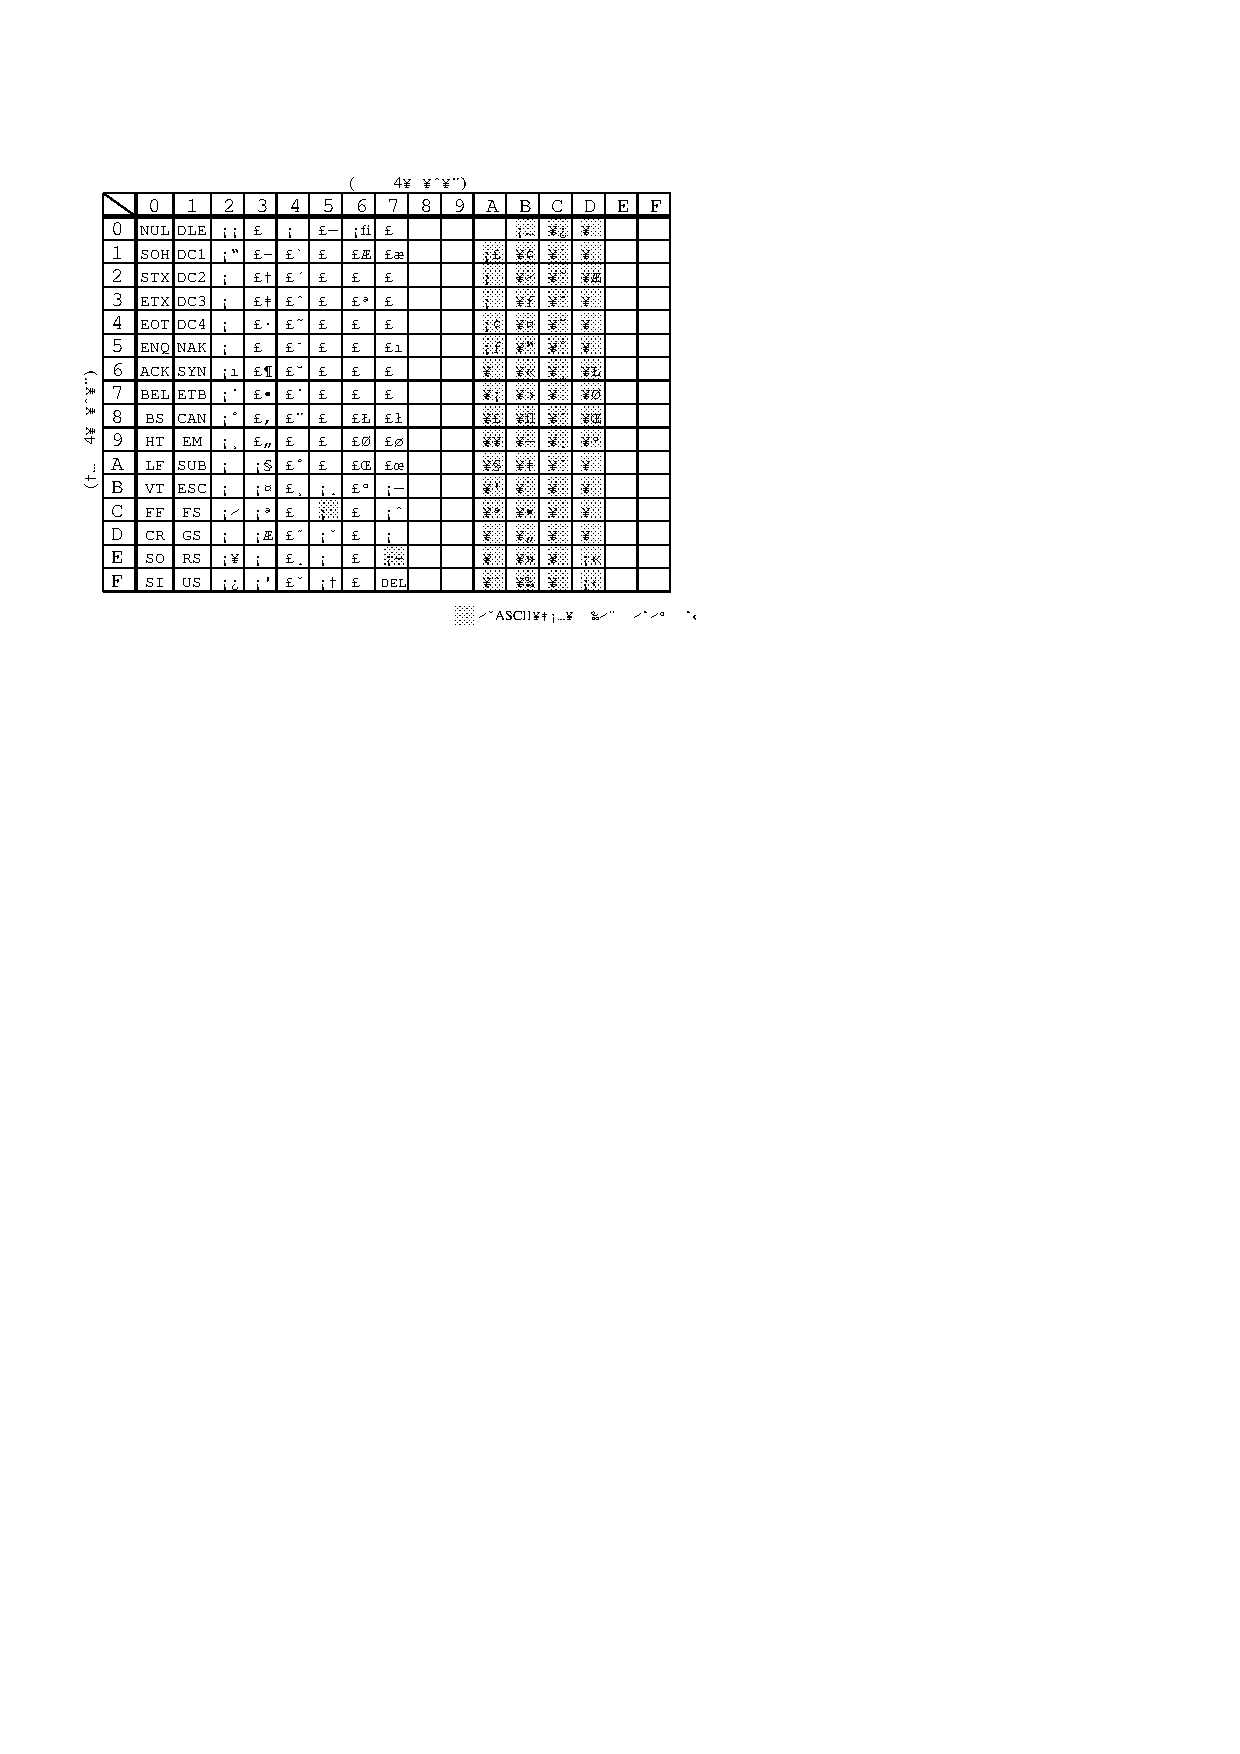
\includegraphics[scale=0.85]{../chap2/jisx0201.pdf}}

\end{frame}

%==============================================================================
\begin{frame}
  \frametitle{文字の表現(Unicode)}
  \emph{Unicode : 最も用いられている業界標準規格}\\
  世界中で使用される全ての文字を収録しようと現在も拡張が続いている.
  \begin{enumerate}
    \item[1.] 全ての文字に21ビットのコードを割り振る.\\
          最大で約111万文字にコードを割り振ることができる.\\
          現在,約15万文字が登録されている.
    \item[2.] 000000H〜00007FHの範囲はASCIIコードと同じ
    \item[3.] 000370H〜0003FFHの範囲にギリシャ文字
    \item[4.] その後に,キリル文字,アルメニア文字,ヘブライ文字...
    \item[5.] 002E80H〜009FFFHの範囲に漢字・かな・カナ・その他
    \item[6.] 00F900H〜00FAFFHの範囲は漢字
    \item[7.] 01F600H〜01F64FHの範囲に顔文字
    \item[8.] 020000H〜0323AFHの範囲も漢字
  \end{enumerate} 
  参考:\url{https://ja.wikipedia.org/wiki/Unicode}
\end{frame}

%==============================================================================
\begin{frame}
  \frametitle{文字の表現(UTF-8)}
  \emph{Unicodeのエンコーディング(符号化)方式の一つ}\\
  21ビットのUnicodeをそのままファイル等に書き込むと,
  00Hのバイトだらけになり容量がもったいないし,
  通信すると時間がかかる. \\
  よく使う文字(ASCII)を短く符号化する.(8ビット可変長)
  \begin{enumerate}
    \item[1.] 000000H〜00007FHの範囲は1バイトに変換 \\
              (00H〜7FH,第1バイトが0で始まる)
    \item[2.] 000080H〜0007FFHの範囲は2バイトに変換  \\
              (C2H,80H〜DFH,BFH,第1バイトが110で始まる)
    \item[3.] 000800H〜00FFFFHの範囲は3バイトに変換 \\
              (E0H,A0H,80H〜EFH,BFH,BFH,第1バイトが1110で始まる)
    \item[4.] 010000H〜10FFFFHの範囲は4バイトに変換 \\
              (F0H,90H,80H,80H〜F7H,BFH,BFH,BFH,第1バイトが11110で始まる)
  \end{enumerate}
  第2バイト以降は,10で始まっている.\\
  参考:\url{https://ja.wikipedia.org/wiki/UTF-8}
\end{frame}

%==============================================================================
\begin{frame}
  \frametitle{補助単位}
  1,000m を 1km,1,000g を 1kg, 0.001 l を 1ml, 0.001m を 1mm\\
  ここで,k や m は\emph{補助単位}と呼ばれる.\\

  \begin{center}
    {\small\begin{tabular}{r l l | r l l}\hline\hline
      \multicolumn{3}{c|}{一般的に} &
      \multicolumn{3}{c}{記憶容量} \\
      \hline
      \multicolumn{1}{c}{値} &
      \multicolumn{1}{c}{記号} &
      \multicolumn{1}{c|}{読み方} &
      \multicolumn{1}{c}{値} &
      \multicolumn{1}{c}{記号} &
      \multicolumn{1}{c}{読み方} \\
      \hline
      $10^3$   & $k$ & キロ   & $2^{10}$ & $Ki$ & キビ \\
      $10^6$   & $M$ & メガ   & $2^{20}$ & $Mi$ & メビ \\
      $10^9$   & $G$ & ギガ   & $2^{30}$ & $Gi$ & ギビ \\
      $10^{12}$& $T$ & テラ   & $2^{40}$ & $Ti$ & テビ \\
    \end{tabular}}
  \end{center}

  \begin{itemize}
  \item 通常は$10^3$毎に補助単位がある.
  \item コンピュータの記憶容量では$2^{10}$毎に補助単位がある.\\
    $2^{10} = 1,024 = 1Ki$ \\
    $10^3   = 1,000 = 1k$
  \end{itemize}
\end{frame}

\end{document}
